\documentclass[journal,12pt]{IEEEtran}
\usepackage{graphicx}
\usepackage{caption}
\usepackage{listings}
\usepackage{algpseudocode}
\usepackage{algorithm}
\usepackage{amssymb}

\lstset{
  basicstyle=\scriptsize\tt,
}

\graphicspath{{figures/}}
\title{Literature Review}
\author{Nicholas Sica}

\begin{document}
\maketitle
Static timing analysis allows a user to analyze circuits and verify
that inputs are arriving at the correct time, taking care not to wipe
away the outputs too quickly. Traditionally, static timing analysis
uses worst, best, and nominal cases to decide on different transistor parameters. While this has
been useful in modeling imperfections in a computationally fast way,
it is not accurate. Block-based static timing analysis allows for a
way to incrementally analyze a circuit. This paper proposes a
block-based approach that allows for uncertainty using different
probability functions. The paper also proposes a novel way to deal
with reconvergent fanouts, an issue that increases complexity
significantly in static timing analysis.

\begin{equation}\label{eq:max_orig}
  A_o = max(A_i + D_{io}, A_j + D_{jo})
\end{equation}

\begin{equation}\label{eq:max}
  C_o = (C_i \circledast P_{io})(C_j \circledast P_{jo})
\end{equation}

\begin{figure}
  \centering
  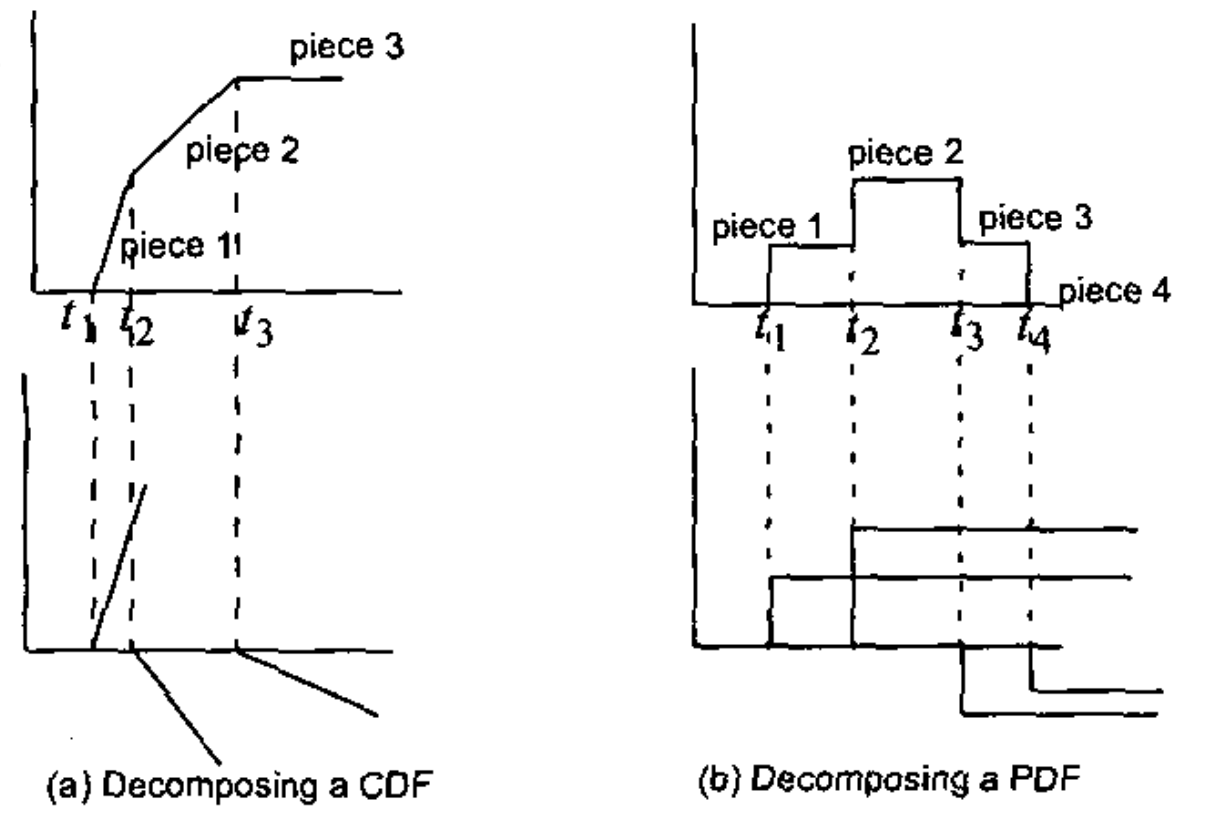
\includegraphics[width=0.95\columnwidth]{decomposed_graphs.png}
  \caption{Decomposing CDF and PDF functions.}\label{fig:decompose}
\end{figure}

In the proposed methodology, arrival times are modeled as cumulative
probability distribution functions~(CDFs) while gate delays are
modeled as probability density functions~(PDFs). While any form can be
used for the CDFs, they use piece-wise linear functions due to ease and
speed of the function type. Typically, the max and operation
used in static timing analysis are given by equation~\ref{eq:max_orig}. In this paper,
convolution and other probability properties are used to determine
these values giving us equation~\ref{eq:max} for max and add. In the equations $A_i$ is the
arrival time at node i,  $A_j$ is the arrival time at node j, $D_{io}$
is the delay between nodes i and o, $D_{jo}$ is the delay between
nodes j and o, $C_i$ is the CDF of node i, $C_j$ is the CDF of node
j, $P_{io}$ is the PDF of $D_{io}$, and $P_{jo}$ is the PDF
of $P_{jo}$. The new equation can be substituted in for the old
equation to get it working right away. Using this new equation
without the reconvergent fanout optimization would yield more accurate
results, but a big performance hit since the computational complexity
is increased by an exponential factor.

The piece-wise linear functions are decomposed as seen in
Fig~\ref{fig:decompose} before they are used in convolutions. The
piece-wise linear functions can be decomposed in a different number of
pieces. The greater the number of pieces, the higher the accuracy of
the static timing analysis. Increasing the number of pieces also
affects the time complexity of the proposed method in an exponential
way.

\begin{equation}\label{eq:mean}
  \mu_x = \mu_z - \mu_y
\end{equation}

\begin{equation}\label{eq:var}
  \sigma_x^2 = \sigma_z^2 - \sigma_y^2
\end{equation}

Reconvergent nets are handled without using path tracing which is
computationally expensive. Instead, the paper uses statistical
subtraction to deal with reconvergent nets. The mean and variance can
be computed directly from the CDF or PDF easily using equation~\ref{eq:mean} and
equation~\ref{eq:var}, respectively. These can then be matched to
determine the distribution in a technique called moment matching. The
algorithm for dealing with all this uses a dependency list to capture
all the vertices in which the current node's arrival time depends
on. This algorithm pseudo-code is shown in Algorithm~\ref{lst:dl_prop}.
We can then further use dependency lists in multi-input gates and expand on
the pseudo-code to create another algorithm as shown in
Algorithm~\ref{lst:reconverge}. This algorithm is used to reduce the
dependency list input to a single vertex to allow for easier use of
the equations discussed earlier.

\begin{algorithm}
  \caption{Propagate dependency list}\label{lst:dl_prop}
  \begin{algorithmic}
    \State $DL_o$ = NULL
    \If{gate output has fanout > 1}
      \State add output node to $DL_o$
    \EndIf
    \For{each input i of gate contributing to output}
      \For{each vertex v in $DL_i$}
        \State add v in $DL_o$ using insertion sort
        \State in descending order by level
      \EndFor
    \EndFor
\end{algorithmic}
\end{algorithm}


\begin{algorithm}
  \caption{Compute arrival time with reconvergent fanout}\label{lst:reconverge}
  \begin{algorithmic}
    \State $A_o$ = -$\infty$
    \For{each input i}
      \State L = NULL
      \For{each vertex v in $DL_i$}
        \If{(V covers more than one input)
            \State $\&\&$ (Y does not appear in L)}
          \State insert Y according to level in L
          \State mark inputs that v covers
        \EndIf
      \EndFor
    \EndFor
    \If{L is empty}
      \State proceed as in independent case
    \Else
      \For{each v in L}
        \State $A_{ov}$ = --$\infty$
        \For{each input i that it covers}
          \State  $A_{ov}$ = max($A_{ov}$, $A_i - A_v + D_{io}$)
        \EndFor
        \State $A_o$ = max($A_o$, $A_{ov}$)
      \EndFor
    \EndIf
    \State return $A_o$
\end{algorithmic}
\end{algorithm}

\begin{figure}
  \centering
  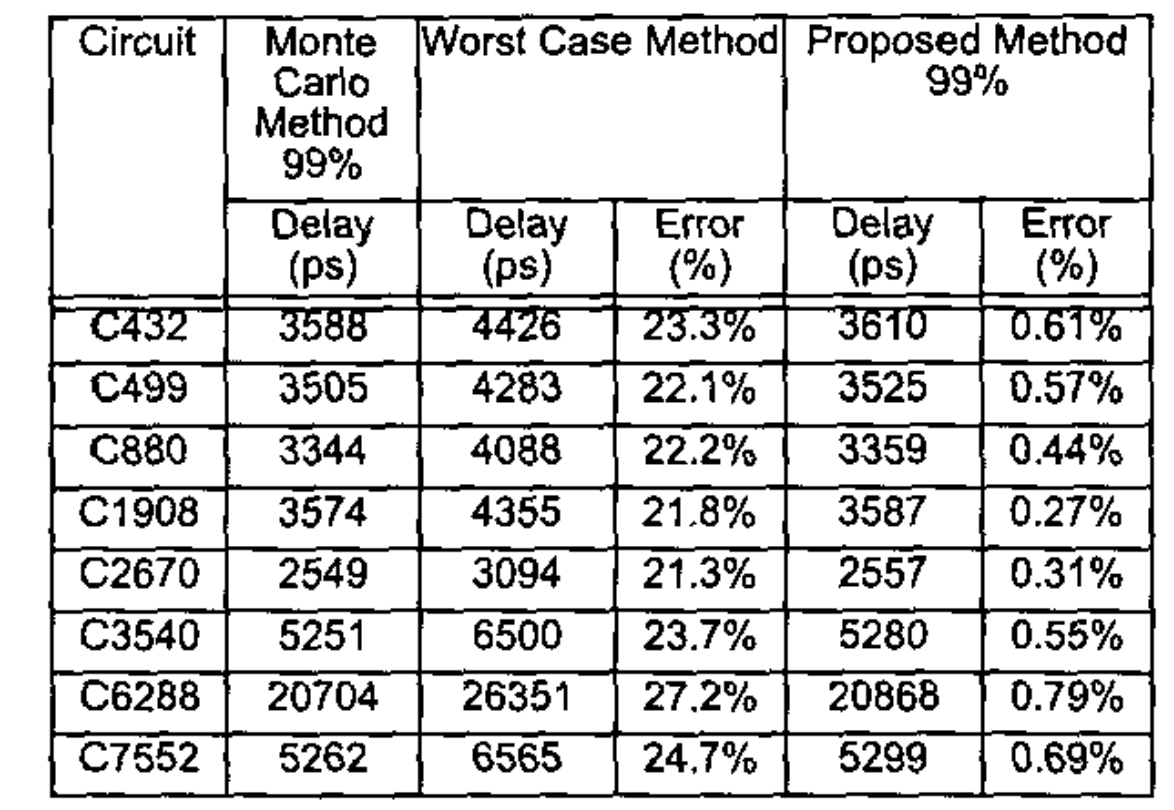
\includegraphics[width=0.95\columnwidth]{results.png}
  \caption{Accuracy comparison of proposed method versus worst case
    and Monte Carlo method.}\label{fig:results}
\end{figure}
The results shown in Fig~\ref{fig:results} show an increase in
accuracy with this new method. Monte Carlo simulations were used as a
golden model to compare against. The results show a peak error of
0.79\% for this new algorithm while a peak error of 27.2\% is shown
for the worst case method. The
lack of numbers to show how long each run took was a bit odd and was a
major point on contention in the paper. Their time complexity is worse
so we should see a hit to speed except in cases where the new
reconvergent fanout algorithm should help it. The lack of speed
numbers makes the conversation about speed and time complexity and
potential speed-ups from the reconvergent fanout algorithm
significantly weaker. They talk about how using the reconvergent
fanout algorithm causes a 10-30\% slowdown over not using it, but
those numbers are not too useful without comparison to current
works. Overall this method could be useful for dealing with
reconvergent nets, but there is not a good way to know for sure
without concrete time numbers to compare if the accuracy increase is
worth the time complexity. Changing the amount of pieces used in the
piece-wise linear function can also increase accuracy but at the cost
of exponentially increasing time complexity. There needs to be more
experimentation in the speed versus accuracy aspects of this proposed
methodology.


%The paper proposes the idea of finding short circuits using a novel
%algorithm to build a tree and feed it into a satisfiability~(SAT)
%solver. Short circuits are when high voltage and ground are
%connected, which can cause a massive current and power spike in the
%system. A satisfiability solver is a program that determines if a
%circuit is satisfiable, which means that there exists a set of inputs
%in which the circuit resolves to a true value. The input to a SAT
%solver is usually a product of sums, an equation that is easy to tell
%when it is false since if any of the clauses are false the entire
%equation is false. When building the graph, it is built in such a way
%that two connected nodes are assumed to have the same value. If the
%two nodes have different values, it would be a short circuit. The
%final formula to be solved is the following~\cite{paper}:
%
%

%\bibliographystyle{IEEEtran}
%\bibliography{ref}

%\begin{figure}
%  \centering
%  \includegraphics[width=0.95\columnwidth]{kmap_unate.png}
%  \caption{A Karnaugh map of a unate problem}\label{fig:kmap_unate}
%\end{figure}
%



%\lstinputlisting[caption=Unate output, label=lst:unate]{unate_output}
%\lstinputlisting[caption=Non-unate output, label=lst:non_unate]{non_unate_output}
%\lstinputlisting[caption=Project problem output, label=lst:example_run]{project_output}
%
%\section{Program}


\end{document}

%%% Local Variables:
%%% mode: latex
%%% TeX-master: t
%%% End:
